\begin{refsection}
	\chapter{Contexte biologique et méthodologique}

    Ce chapitre présente les notions, biologiques puis informatiques, utilisées comme fondement du travail de recherche, effectué lors de cette thèse.
    
    
    \section{Le métabolisme et sa représentation informatique}
    \subsection{Généralités sur le métabolisme}
    
    Tout organisme vivant, consomme de l'énergie afin de perpétuer son espèce. Pour cela, l'être vivant doit assimiler des composés présent dans son environnement. Ces composés chimiques permettent de produire l'énergie, nécessaire à la survie mais surtout à la transmission du patrimoine génétique. Ainsi on désigne par métabolisme, l'ensemble des processus de synthèse et dégradation de composé chimique, mis en œuvre par l'organisme. De fait, les processus comme la réplication de l'\gls{ADN}, la traduction d'un gène et autres \ldots~sont exclus.
    
    \note{Le mot métabolisme à évolué à travers l'histoire pour nous parvenir sous ça forme actuelle. En grec ancien on utilisé "\greekFont{μεταβολή}" équivalent à metabolé désignant "transformation". Le mot métabole signifie "qui subit un changement". Il a été utilisé par la suite comme mot racine: métabol-ique, métabol-isme \ldots
    }
    
    Les organismes vivant opèrent une multitude de transformations chimiques. Elles forment de véritable usine de traitement biochimique. En effet, elles disposent d'une batterie de réaction biochimique, afin de traité un grand nombre de composés, tant à l'intérieur qu'à l'extérieur de la cellule. Par exemple, certains composés, de par la nature de la membrane cellulaire\footnote{La membrane cellulaire constitue une barrière physique entre le milieu extérieur et  intérieur de la cellule.}, doivent être transformé depuis l'extérieur de la cellule, afin d'assimiler le composé transformé. De ce fait, la matière présente dans l'environnement est utilisé pour constituer les briques nécessaires au vivant.
    
    Par conséquent, le métabolisme est essentiel à la vie, d'une part il fournit l'énergie nécessaire. Et d'autre part, il va produire les molécules de base indispensables à l'organisme, pour sa construction, sa défense et autres \ldots 
    
    Bien qu'agissant à une échelle moléculaire, le métabolisme d'un groupe d'organisme peut impacter son environnement. Si bien que les conséquences peuvent être observées à l'échelle humaine voire dans certains cas à l'échelle de la planète (voir Figure~\ref{fig:bloom}). Un autre exemple est celui des espèces végétales. Ils absorbent du dioxyde de carbone et produisent de l'oxygène. Ainsi ils jouent un rôle important dans la concentration de ces composés dans l’atmoshpère.
    
    
    \begin{shadedfigure}
        \begin{subfigure}[b]{.5\textwidth}
            \centering
            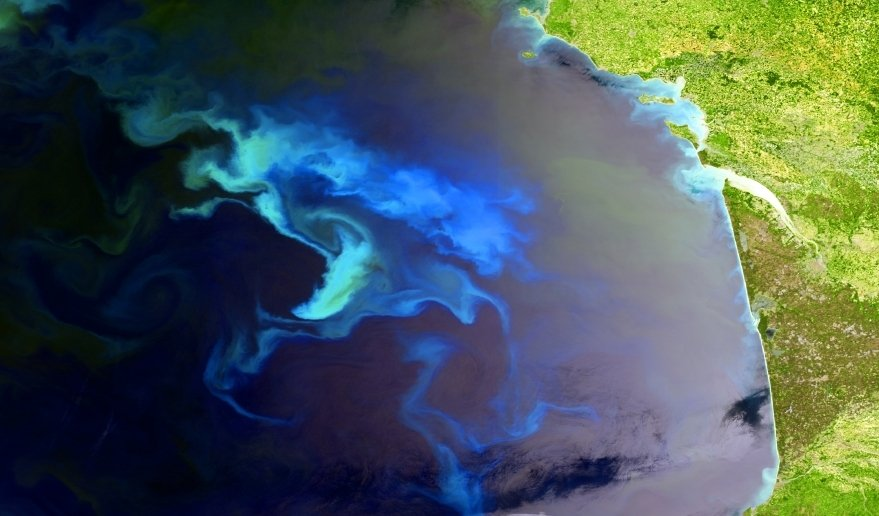
\includegraphics[width=\textwidth]{img/bloom_gascogne.jpg}
            \caption{{\tiny Source: \url{http://seos-project.eu}}}
            \label{fig:bloom_gascogne}
        \end{subfigure}
        \hfill
        \begin{subfigure}[b]{.5\textwidth}
            \centering
            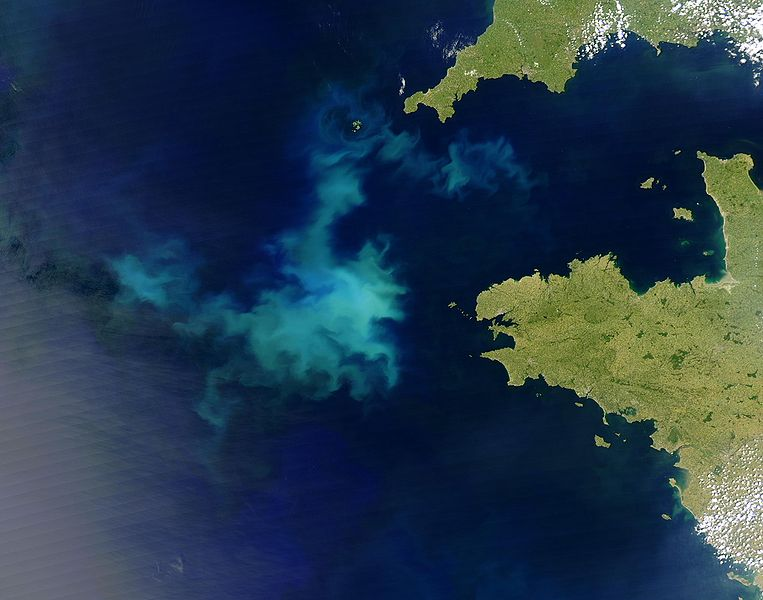
\includegraphics[width=\textwidth]{img/bloom_bretagne.jpg}
            \caption{{\tiny Source: \url{https://commons.wikimedia.org/}}}
            \label{fig:bloom_bretagne}
        \end{subfigure}
    \caption{Le métabolisme d'un groupe d'individu produit une quantité de pigment photosynthétiques suffisamment conséquente, qu'il en devient observable depuis l'espace. Deux évènements distinct sont représentés. Le premier a eu lieu au large de la Gascogne le 17 mai 2004 et le second au niveau de la Bretagne le 15 juin 2004.}
    \label{fig:bloom}
    \end{shadedfigure}

	\note{Lors de l'apparition des premières formes de vie, il y a 3,6 milliards d’années. L'atmosphère était faiblement pourvue en oxygène. Ces organismes anaérobiques était présent dans les océans. L'oxygène est toxique, leur métabolise s'est adapté au dioxyde de carbone, présent abondamment à ce moment. Puis entre 3.5 à 3 milliard apparurent des cyanobactéries. Ce sont des bactéries photosynthétiques. Leur métabolisme a la particularité d'oxyder les minéraux  présent dans les océans. Ils produisent ainsi de l'oxygène. Avec le temps leur métabolisme à consommé tellement de minéraux que l'oxygène produits dans les océans est libéré dans l’atmosphère. Modifiant ainsi fortement ça composition. Cet évènement influença le cours de la vie. De sorte que des organismes s'adaptent à l'oxygène. Car l'oxygène devient une molécule courante. Certaine forme de vie évolua jusqu'a devenir aérobie. La Terre a subit ça première pollution atmosphérique d'ampleur induit par des organismes vivant.}
    
    L'étude du métabolisme est essentiel pour la compréhension des êtres vivants. Les débouchés impacte de nombreux domaines, tel que : la pharmaceutique, l'énergie, l'agriculture, l'environnement \ldots . Afin de mieux appréhender les notions sous-jacentes aux métabolismes, la section suivante introduit les acteurs du métabolisme, les agents impliqués, ainsi que la notion de réaction.

    \subsection{Les acteurs}
    
    On distingue dans le métabolisme deux catégories de processus, l'anabolisme et le catabolisme. L'anabolisme, représente l'ensemble des réactions impliqué dans la synthèse de nouvelle molécule. La production de nouveaux composés nécessite de l'énergie. De tels processus sont composés de réaction endergonique. Ainsi le bilan énergétique est négatif.  Au contraire, le catabolisme décrit l'ensemble des réactions de dégradation de molécule. Les réactions impliquées dans la dégradation d'une composé, produisent in-fine plus d'énergie qu'elles en on consommé. Ces réactions produisant de l'énergie sont dites exergoniques.
    
    \subsubsection{Les métabolites}
    
    La succession des différents processus issus du métabolisme, produit des composés organiques intermédiaires, de petite taille, appelé métabolite. Ils sont tour à tour synthétisés puis dégradés. Selon leurs rôles, ils interviennent soit dans les processus indispensables au développement et à la reproduction, dit "métabolisme primaire" . Soit à des fonctions non vitale comme la production d'antibiotique, de phéromone, de pigment \ldots, dénommé "métabolisme secondaire" .
    
    \note{Un composé organique s'oppose a un composé minéral. Cette différentiation s'explique par des raisons philosophiques antérieur au \siecle{19}. En effet, on distinguait les substances constitutives des organismes des autres. Ne sachant pas synthétisé les molécules organiques. On expliquait qu'elle nécessité l'intervention d'une "force vitale". En 1828, Friedrich Wöler mis au point, accidentalement une expérience, produisant de l'urée (considéré comme organique) à partir de composé minéraux, comme le cyanate d’ammonium. Depuis lors, la notion de composé organique a évolué afin de désigné une molécule consitué d'une partie de carbone, le reste pouvant être des atomes d'hydrogène, oxygène azote et autres \ldots. La notion organique est resté car le carbone est un élément essentiel du vivant. Par opposition un composé minéral correspond à toutes toutes molécules constitué d'élément autre que le carbone. Pour plus d'information, je vous invite à lire \citetitle{chimie_organique}.
    }
    
    
    \subsubsection{Les cofacteurs}
    ATP ADP energie
    
    
    \subsubsection{Les réactions}
    Ces processus s'effectuent au sein de l'organisme, dans l'infiniment petit, au niveau moléculaire. Effectivement des molécules produites par l'organisme vont avoir une affinité avec des composés chimiques. Leur rencontre provoque une transformation du composé. Puis, le ou les produits résultant de cette transformations, peuvent êtres à leur tour reconnu par des molécules produites par l'organisme. Provoquant ainsi une cascade de transformation chimique.
    
    \subsection{Représentation en graphe}
    \subsection{Ressources sur les voies métaboliques}
    \subsubsection{KEGG}
    \subsubsection{Reactome}
    \subsubsection{Unipathway}
    \subsubsection{Genome properties}
    
    \section{Des génomes aux réseaux métaboliques}
    \subsection{Annotation fonctionnelle}
    \subsection{Reconstruction des réseaux métaboliques}
    \subsection{Modèles métaboliques}
    \subsection{Les données expérimentales}
    \subsubsection{Élucidation des voies métaboliques}
    \subsubsection{Phénotypes de croissances}
    
    \section{Raisonnement logique dans le processus de curation}
    \subsection{Lacunes et incertitudes dans nos connaissances}
    \subsubsection{Les trous dans les connaissances et les enzymes orphelines}
    \subsubsection{Limites de l’annotation fonctionnelle et rôle de la curation}
    \subsection{Logique et raisonnement}
    \subsubsection{Les différentes logiques}
    \paragraph{Logique booléenne}
    \paragraph{Logique multi-valuée}
    \subsubsection{Inférence d’information}
    \paragraph{Représenation des connaissances/ontologies}
    \paragraph{Chainage avant et arrière} %backward/forward
    \paragraph{Règles et système expert}
    
    \section{Méthodes existantes}
    \subsection{HAMAP et UniRule}
    \subsection{Genome properties}
    \subsection{IMG terms}
    \subsection{HERBS}
    
    \subbibliography
\end{refsection}